%!TEX root = ../main.tex
\setcounter{chapter}{7}
\setcounter{section}{0}
\section{Digitization}
\vspace{-8pt} \hrule \hrule \hrule \hrule \hrule  \vspace{12pt}

$\bigstar$ Sampling Process
	    \begin{figure}[!h]
	        \centering
	        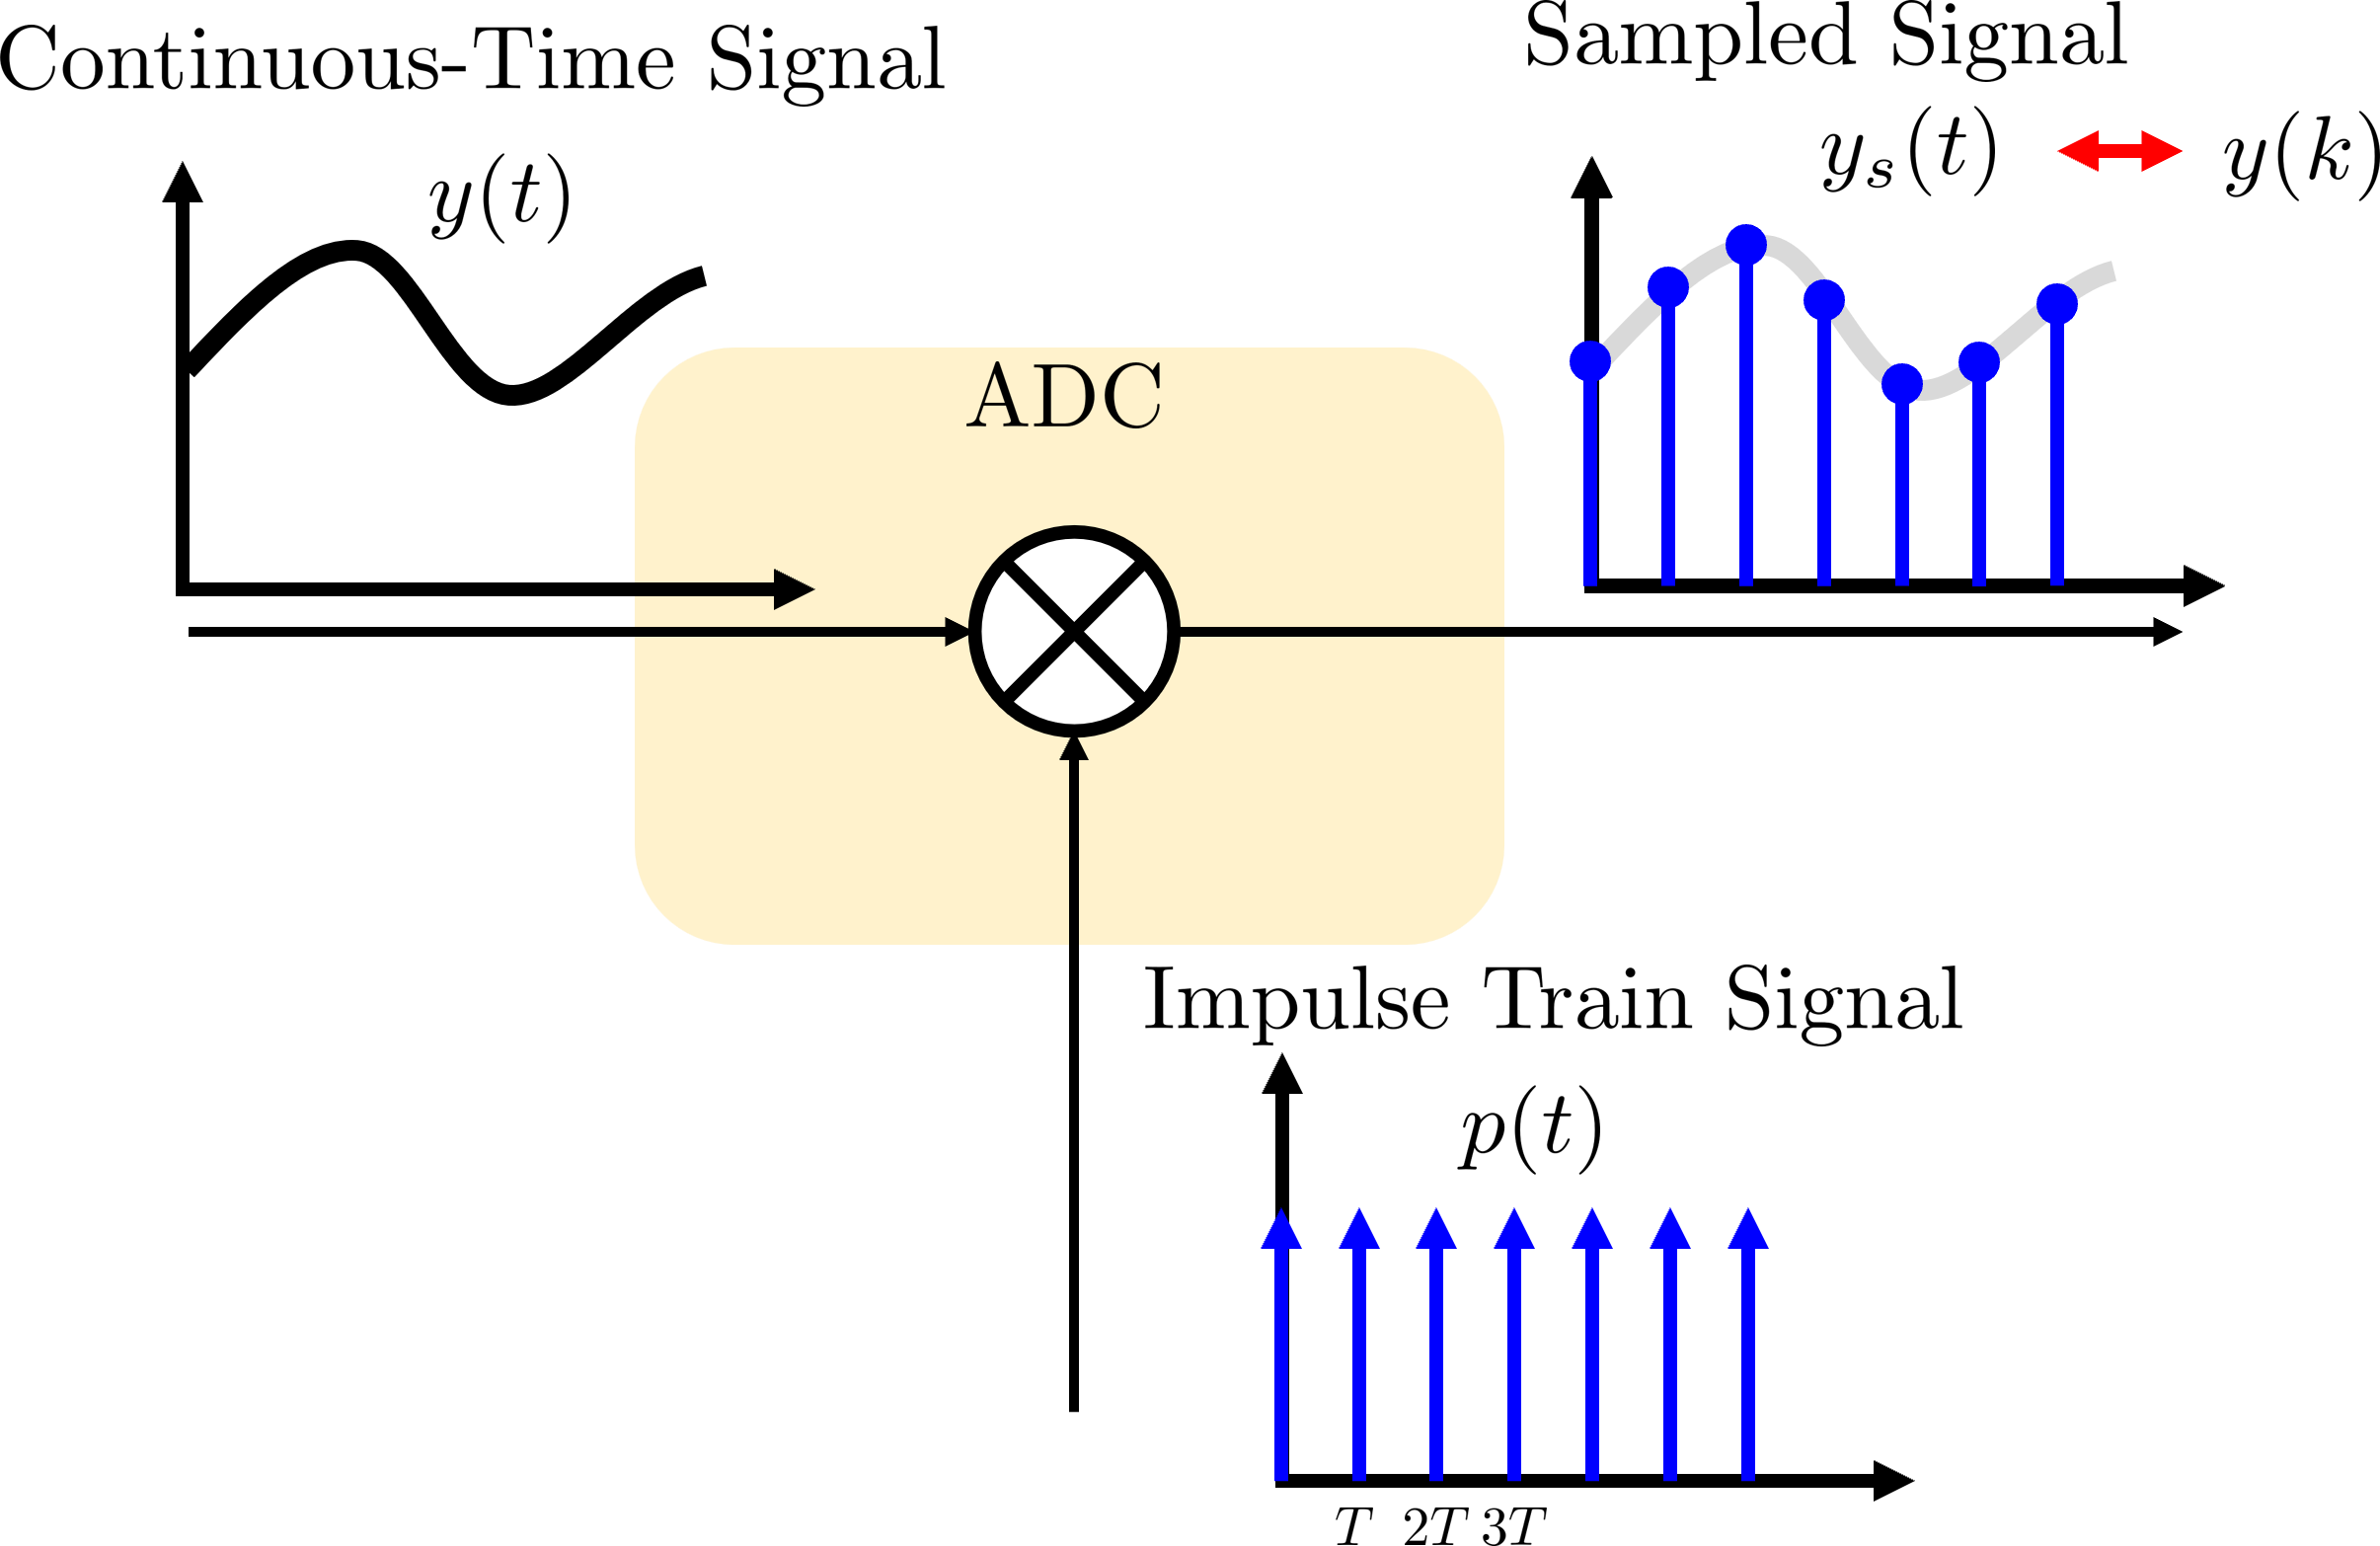
\includegraphics[width=10cm]{./FIG_Franklin/fig8-smc3.png}
	    \end{figure}
    \begin{enumerate}
    	\item Periodic Impulse Train: p(t) is periodic with period $T = 1/F_s$
    	\begin{align*}
    		p(t) = \sum_{k=-\infty}^{\infty} \delta(t-kT)
    	\end{align*}
     	\item Sampled Signal: we can consider $y_s(t)$ te be the analog equivalent to discrete-time signal $y(k)$ or $y(kT)$
    	\begin{align*}
    		y_s(t) &= y(t) \cdot p(t) = \sum_{k=-\infty}^{\infty} y(t)\delta(t-kT) = \sum_{k=-\infty}^{\infty} y(kT)\delta(t-kT)\\
    			&\leftrightarrow y(k) = y(kT)
    	\end{align*}
	\end{enumerate}